\documentclass{beamer}
\usepackage[utf8x]{inputenc}
\usepackage[czech]{babel}
\usetheme[pageofpages=of,% String used between the current page and the
                         % total page count.
          bullet=circle,% Use circles instead of squares for bullets.
          titleline=true,% Show a line below the frame title.
	  titlepagelogo=opensuse,
          alternativetitlepage=true,% Use the fancy title page.
          ]{Torino}

\setbeamerfont{title}{series=\bfseries,size=\LARGE}
\author{Tom\'{a}\v{s} Chv\'{a}tal\newline {\small openSUSE Team}}
\title{Whats new in LibreOffice 4.1 and whats comming}
\date{2013/07/20}

\begin{document}

\begin{frame}[t,plain]
\titlepage
\end{frame}

\section{Introduction}

\begin{frame}[t]{Who the hell is Tomáš Chvátal}
	\begin{itemize}
	\item SUSE Employee since 2011 (QA, openSUSE)
	\item Packager of Libreoffice and various other stuff for openSUSE
	\item openSUSE promoter and volunteer
	\item Gentoo developer since fall 2008 and Council member since 2010
	\end{itemize}
\end{frame}

\section{Libreoffice 4.1 features}

\subsection{Writer features}

\begin{frame}[t]{Fonts embedding}
	\begin{itemize}
	\item Feature apply actually for all parts, writer/impress/calc/...
	\item Ensures that your peers can see the document exactly like you
	\item Applies only for OpenDocument formats
	\item File $\rightarrow$ Properties $\rightarrow$ Font $\rightarrow$ Embedd fonts in the document
	\end{itemize}
\end{frame}

\begin{frame}{90 Degree rotation of images}
	\begin{figure}
	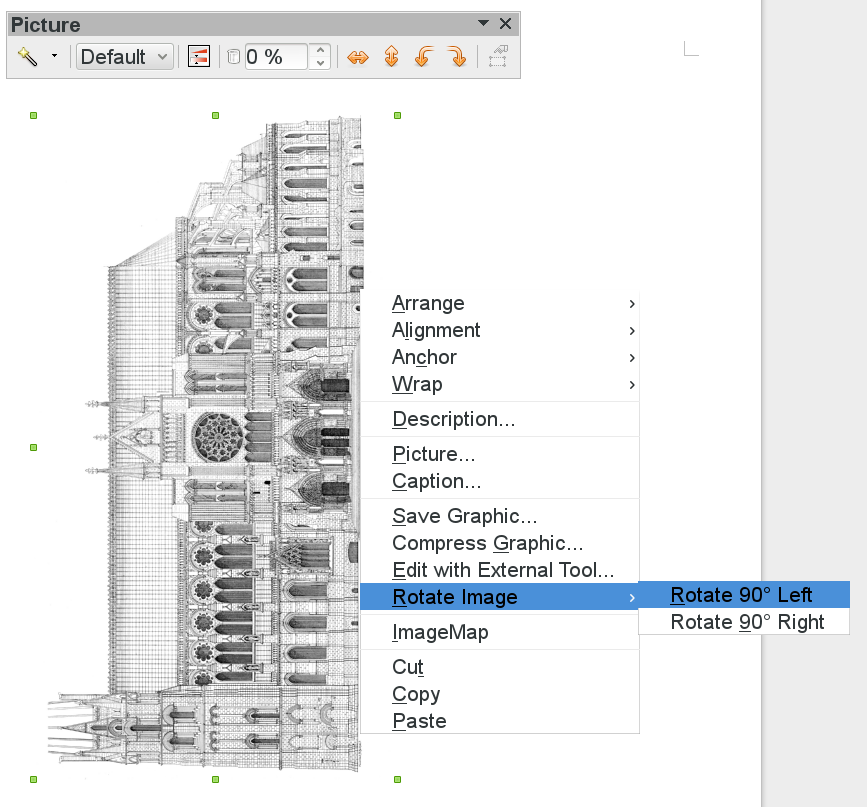
\includegraphics[width= 0.6\linewidth]{90degreerotation-writer.png}
	\end{figure}
\end{frame}


\begin{frame}{Gradient background}
	\begin{figure}
	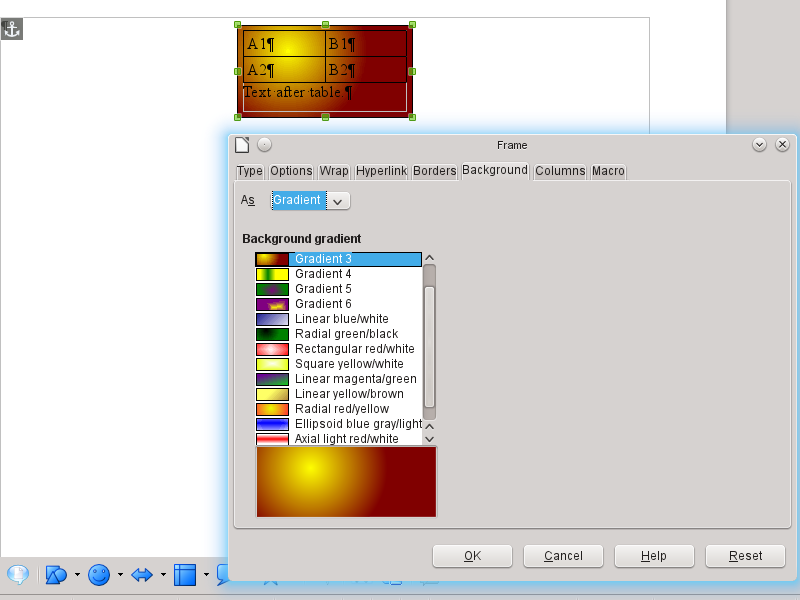
\includegraphics[width= 0.8\linewidth]{gradientbg-writer.png}
	\end{figure}
\end{frame}

\begin{frame}{Range comments can span multiple paragraphs}
	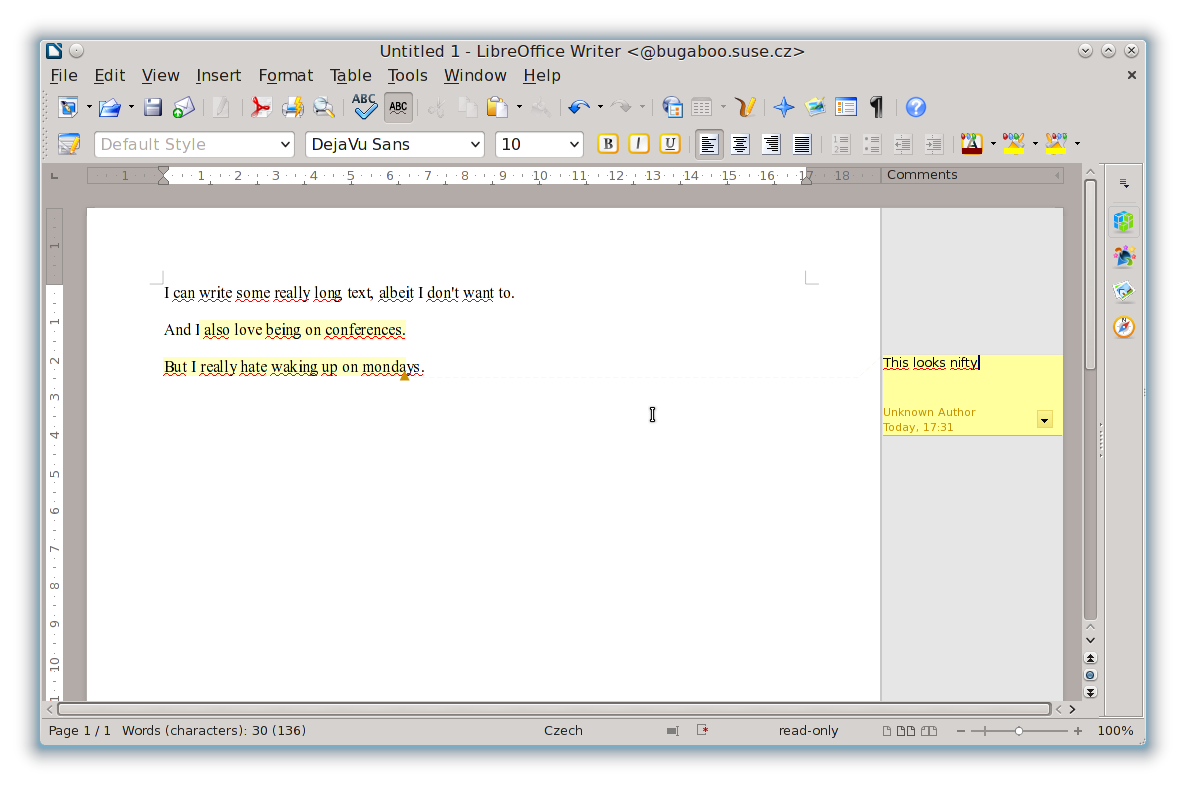
\includegraphics[width= 1.0\linewidth]{rangecomments-writer.png}
\end{frame}

\subsection{Calc features}

\begin{frame}[t]{Large tables import support $>$64k table cells}
	\begin{itemize}
	\item With this fuction you can finally put in use huge stylesheet
	\item The problem was that previously with big sheets you imported only 13635 from word file and lost the rest silently
	\item Big problem is that calc is just huge mesh of cells, which inflict speed problems with more and more cells in equasion (this is being fixed if I am not mistaken)
	\end{itemize}
\end{frame}

\begin{frame}[t]{New functions from excel 2013 for formulas creation}
ACOT, ACOTH, ARABIC, BASE, BINOM.DIST.RANGE (B) [BINOM.DIST.RANGE], BITAND, BITLSHIFT, BITOR, BITRSHIFT, BITXOR, COMBINA, COT, COTH, CSC, CSCH, DAYS, DECIMAL, FORMULATEXT (FORMULA) [FORMULA], GAMMA, GAUSS, IFNA, IMCOSH, IMCOT, IMCSC, IMCSCH, IMSEC, IMSECH, IMSINH, IMTAN, ISFORMULA, MUNIT, NUMBERVALUE, PDURATION (DURATION) [PDURATION], PERMUTATIONA, PHI, RRI, SEC, SECH, SHEET, SHEETS, SKEW.P (SKEWP) [SKEWP], UNICHAR, UNICODE, XOR
\end{frame}

\begin{frame}{Counting selected cells}
	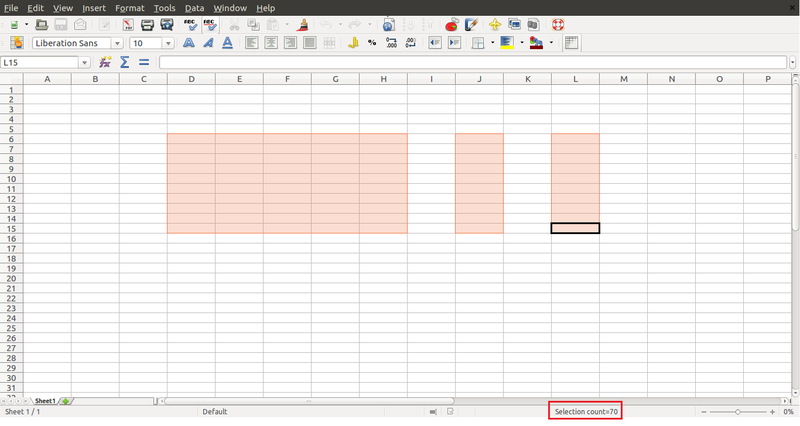
\includegraphics[width= 1.0\linewidth]{cells-selection-count-calc.png}
\end{frame}

\subsection{Impress features}

\begin{frame}[t]{Creating picture series presentations}
	\begin{itemize}
	\item Family reunions were never scarier
	\item Just point impress to folder with photos and you get series of your pictures for everyone
	\item Insert $\rightarrow$ Picture $\rightarrow$ Photo Album
	\end{itemize}

\end{frame}

\subsection{Base features}

\begin{frame}{LIMIT for results}
	\begin{center}
	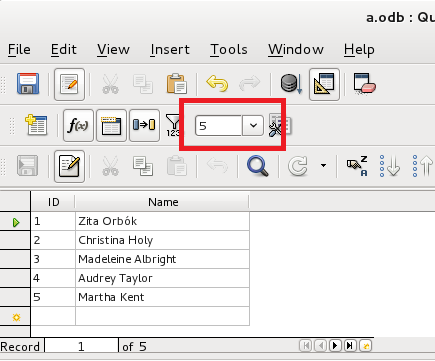
\includegraphics[width= 0.7\linewidth]{limit-base.png}
	\end{center}
\end{frame}

\subsection{Global/Core changes}

\begin{frame}[t]{Core changes}
	\begin{itemize}
	\item There is ongoing effort punting java in favor of python, tis time Agenda and Web wizzards were pythonified
	\item Text rendering was moved from deprecated ICU LE to HarfBuzz (mostly used up now in chrome)
	\item More dialogs were rewritten with HIG in mind (glade .ui files).
	\item New Galery images from Lotus Symphony
	\item Experimental sidebar from Lotus Symphony, this is being converted to dynamic expansion and the feature should be completely ready for 4.2 release.
	\end{itemize}
\end{frame}

\begin{frame}[t]{Core changes: part 2}
	\begin{itemize}
	\item Deprecation of dmake
	\item Reduction of german comments (around 17k lines, 3.3 had 52k)
	\item Tons of coverity fixes
	\item Automated detection of crasher bugs
	\item 100+ new unit tests to cover more ground
	\item Complete SDF removal -> way faster build with enabled languages
	\end{itemize}
\end{frame}

\subsection{Filter updates}

\begin{frame}[t]{New provider for mwaw format}
	\begin{itemize}
	\item Files generated on Mac OS (pre-OSX)
	\item Microsoft Word for Mac 5.1, Write Now 4.0, MacWrite Pro 1.5, Appleworks 6.0
	\item Even if questionable use nowdays it is always good to be able to open old documents
	\end{itemize}
\end{frame}

\subsection{Help updates}

\begin{frame}{Syntax highlighting}
	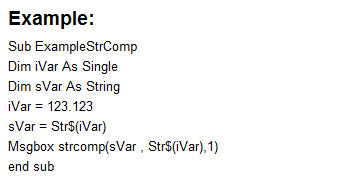
\includegraphics[width= 0.5\linewidth]{syntax36-help.png}
	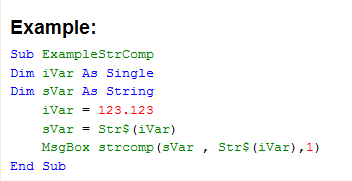
\includegraphics[width= 0.5\linewidth]{syntax41-help.png}
\end{frame}

\section{Contributing}

\subsection{Graphs}

\begin{frame}{Current contributors}
	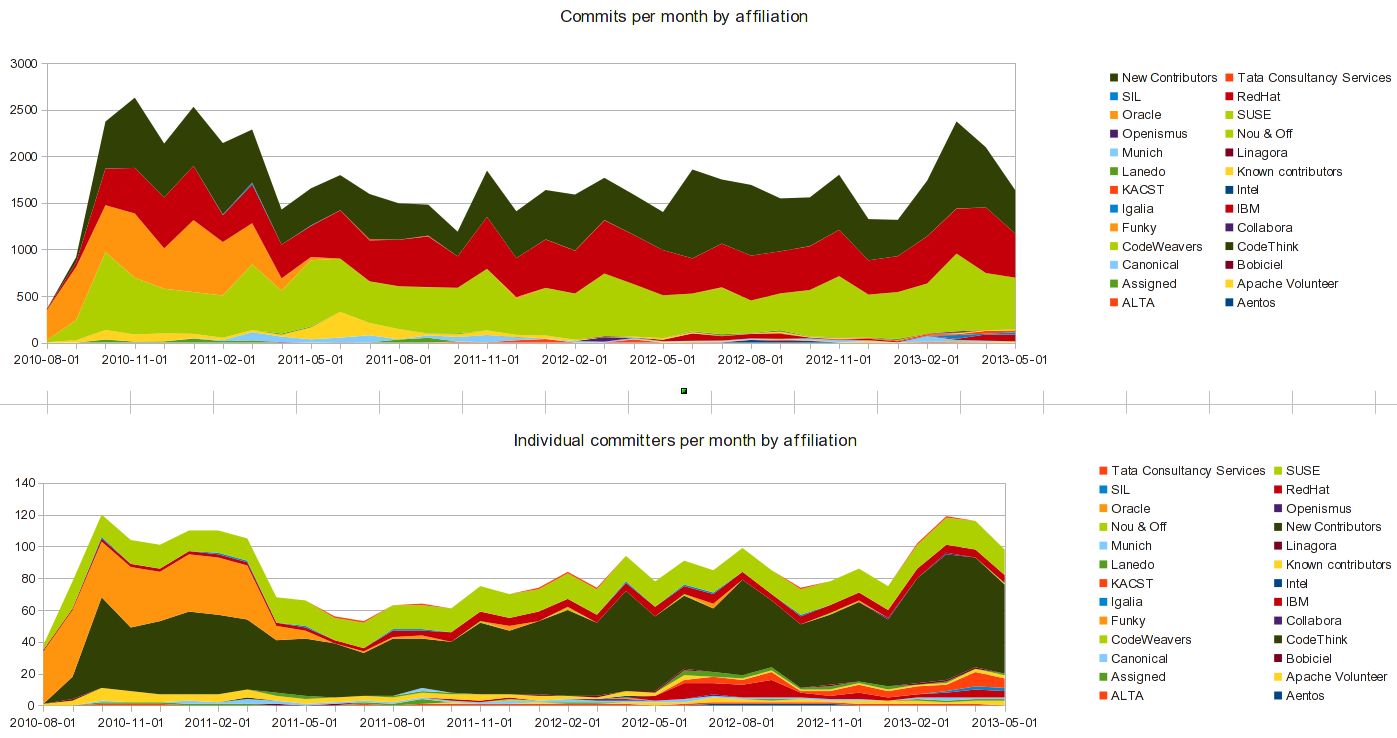
\includegraphics[width= 1.0\linewidth]{contribution-graph.png}
\end{frame}

\begin{frame}{Unique hits on page per version}
	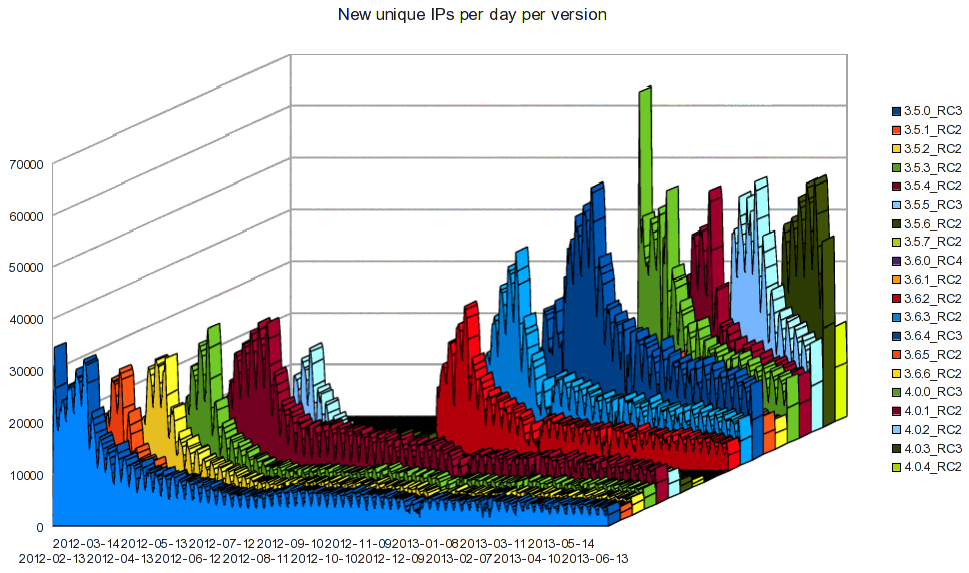
\includegraphics[width= 1.0\linewidth]{downloads-unique.png}
\end{frame}

\subsection{How can I contribute}

\begin{frame}[t]{Working with bugs}
	\begin{itemize}
	\item Report your bugs using assistant https://www.libreoffice.org/get-help/bug/
	\item Work in bugzilla to confirm and cleanup all the reported bugs
	\item Currently there are 5442 overall open bugs, weekly it gets around 200 more and around 100 is closed
	\end{itemize}
\end{frame}

\begin{frame}[t]{Running tinderbox}
	\begin{itemize}
	\item Tool running continuous builds to see if something broke or not
	\item http://tinderbox.libreoffice.org/MASTER/status.html
	\item Even if it is without fancy css it provides great fast way how to keep the code compiling under various build setups
	\end{itemize}
\end{frame}

\section{Thanks}

\begin{frame}{Suse is hiring}
	\begin{figure}
	
\includegraphics[width= 0.8\linewidth]{suse_hiring.png}
	\end{figure}
\end{frame}

\begin{frame}{Questions}
	\begin{center}
	Any curious questions? Did I forget your favorite new feature?
	\end{center}
\end{frame}

\begin{frame}{Thanks}
	\begin{center}
	Thank you for your attention.
	\end{center}
\end{frame}

\end{document}

